% Chapter 1

\chapter{Introducción general} % Main chapter title

\label{Chapter1} % For referencing the chapter elsewhere, use \ref{Chapter1} 
\label{IntroGeneral}

Un sistema de control de actitud (ADCS, por sus siglas en inglés Attitude Determination and Control System) es un conjunto de componentes de hardware y software que permite a un objeto, como un satélite o una nave espacial, mantener o modificar su orientación en el espacio. Para realizar cambios en su orientación, el sistema utiliza actuadores. Un actuador es un dispositivo físico que genera movimiento o aplica una fuerza para producir un cambio en la posición o dirección de un objeto.Para lograr su funcionamiento, el sistema combina tres funciones principales:

\begin{enumerate} 
	\item Medición de la orientación actual mediante sensores. 
	\item Procesamiento de estos datos para estimar la orientación mediante algoritmos. 
	\item Aplicación de correcciones de orientación mediante actuadores. \end{enumerate}

Estas correcciones buscan minimizar la diferencia entre la orientación actual y la deseada, asegurando que el objeto mantenga la orientación requerida con precisión. Este tipo de sistemas se emplea en vehículos espaciales, drones, sistemas de estabilización de cámaras fotográficas, entre otros.


%----------------------------------------------------------------------------------------

% Define some commands to keep the formatting separated from the content 
\newcommand{\keyword}[1]{\textbf{#1}}
\newcommand{\tabhead}[1]{\textbf{#1}}
\newcommand{\code}[1]{\texttt{#1}}
\newcommand{\file}[1]{\texttt{\bfseries#1}}
\newcommand{\option}[1]{\texttt{\itshape#1}}
\newcommand{\grados}{$^{\circ}$}

%----------------------------------------------------------------------------------------

%\section{Introducción}

%----------------------------------------------------------------------------------------
\section{CONTROL DE ACTITUD}
En la actualidad existen pequeños satélites que orbitan alrededor de la tierra denominados CubeSats. Estos tienen componentes electrónicos modulares, donde uno de estos módulos se llama ADCS. El sistema ADCS se encarga de mantener y corregir  la orientación del satélite mediante un algoritmo de control, a una orientación deseada.

Un sistema ADCS consta de una unidad inercial (IMU por sus siglas en inglés). Este dispositivo mide el campo magnético, aceleración y velocidad angular en tres ejes. A partir de estos datos  obtiene la orientación y orientación dentro del espacio usando una variedad de algoritmos conocidos (TRIAD,Davenports,etc).  A partir de alguno de estos algoritmos se genera una actuación sobre  el sistema para que el cubesat pueda mantener la orientación en el espacio. La forma de mantener la orientación en el espacio es aplicar una fuerza conocida, esta produce un torque (o par) en alguno de los ejes principales y mantiene la orientación respecto de perturbaciones externas.

\section{Desarrollo del trabajo}
	El presente trabajo consiste en desarrollar la simulación de un control de actitud mediante el algoritmo TRIAD. Este utiliza como entradas del mismo, dos referencias conocidas, y dos estimadas y a partir de ellas puede obtiene la orientación. El diagrama en bloques del trabajo que se desarrolla se muestra a continuación: 
	\begin{figure}[htbp]
		\centering
		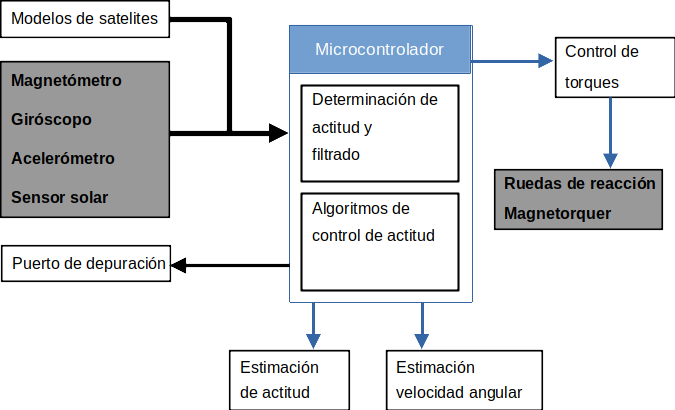
\includegraphics[width=\textwidth]{./Figures/sistemaadcs.png}
		\caption{Diagrama en bloques del trabajo desarrollado.}
		\label{fig:simulate_sistem}
	\end{figure}

\section{Objetivos}

Acá tiene un ejemplo de una ``subsubsección'' que es el cuarto nivel de ordenamiento del texto, después de capítulo, sección y subsección.  Como se puede ver, las subsubsecciones no van numeradas en el cuerpo del documento ni en el índice.  El formato está definido por la plantilla y no debe ser modificado.

\subsection{Guía matemática rápida para \LaTeX{}}

Si estás escribiendo un documento con mucho contenido matemático, entonces es posible que desees leer el documento de la AMS (American Mathematical Society) llamado, \enquote{A Short Math Guide for \LaTeX{}}. Se puede encontrar en línea en el siguiente link: \url{http://www.ams.org/tex/amslatex.html} en la sección \enquote{Additional Documentation} hacia la parte inferior de la página.


%----------------------------------------------------------------------------------------

\section{Utilizando esta plantilla}

Si estás familiarizado con \LaTeX{}, entonces podés explorar la estructura de directorios de esta plantilla y proceder a personalizarla agregando tu información en el bloque \emph{INFORMACIÓN DE LA PORTADA} en el archivo \file{memoria.tex}.  

Se puede continuar luego modificando el resto de los archivos siguiendo los lineamientos que se describen en la sección \ref{sec:FillingFile} en la página \pageref{sec:FillingFile}.

Debés asegurarte de leer el capítulo \ref{Chapter2} acerca de las convenciones utilizadas para las Memoria de los Trabajos Finales de la \degreename.

Si sos nuevo en \LaTeX{}, se recomienda que continúes leyendo el documento ya que contiene información básica para aprovechar el potencial de esta herramienta.


%----------------------------------------------------------------------------------------

\section{Qué incluye esta plantilla}

\subsection{Carpetas}

Esta plantilla se distribuye como una único archivo .zip que se puede descomprimir en varios archivos y carpetas. Asimismo, se puede consultar el repositorio git para obtener la última versión de los archivos, \url{https://github.com/patriciobos/Plantilla-CESE.git}. Los nombres de las carpetas son, o pretender ser, auto-explicativos.

\keyword{Appendices} -- Esta es la carpeta donde se deben poner los apéndices. Cada apéndice debe ir en su propio archivo \file{.tex}. Se incluye un ejemplo y una plantilla en la carpeta.

\keyword{Chapters} -- Esta es la carpeta donde se deben poner los capítulos de la memoria. Cada capítulo debe ir un su propio archivo \file{.tex} por separado.  Se ofrece por defecto, la siguiente estructura de capítulos y se recomienda su utilización dentro de lo posible:

\begin{itemize}
\item Capítulo 1: Introducción general	
\item Capítulo 2: Introducción específica
\item Capítulo 3: Diseño e implementación
\item Capítulo 4: Ensayos y resultados
\item Capítulo 5: Conclusiones

\end{itemize}

Esta estructura de capítulos es la que se recomienda para las memorias de la especialización.

\keyword{Figures} -- Esta carpeta contiene todas las figuras de la memoria.  Estas son las versiones finales de las imágenes que van a ser incluidas en la memoria.  Pueden ser imágenes en formato \textit{raster}\footnote{\url{https://en.wikipedia.org/wiki/Raster_graphics}} como \file{.png}, \file{.jpg} o en formato vectoriales\footnote{\url{https://en.wikipedia.org/wiki/Vector_graphics}} como \file{.pdf}, \file{.ps}.  Se debe notar que utilizar imágenes vectoriales disminuye notablemente el peso del documento final y acelera el tiempo de compilación por lo que es recomendable su utilización siempre que sea posible.

\subsection{Archivos}

También están incluidos varios archivos, la mayoría de ellos son de texto plano y se puede ver su contenido en un editor de texto. Después de la compilación inicial, se verá que más archivos auxiliares son creados por \ LaTeX{} o BibTeX, pero son de uso interno y no es necesario hacer nada en particular con ellos.  Toda la información necesaria para compilar el documento se encuentra en los archivos \file{.tex}, \file{.bib}, \file{.cls} y en las imágenes de la carpeta Figures.

\keyword{referencias.bib} - este es un archivo importante que contiene toda la información de referencias bibliográficas que se utilizarán para las citas en la memoria en conjunto con BibTeX. Usted puede escribir las entradas bibliográficas en forma manual, aunque existen también programas de gestión de referencias que facilitan la creación y gestión de las referencias y permiten exportarlas en formato BibTeX.  También hay disponibles sitios web como \url{books.google.com} que permiten obtener toda la información necesaria para una cita en formato BibTeX. Ver sección \ref{sec:biblio}

\keyword{MastersDoctoralThesis.cls} -- este es un archivo importante. Es el archivos con la clase que le informa a \LaTeX{} cómo debe dar formato a la memoria. El usuario de la plantilla no debería necesitar modificar nada de este archivo.

\keyword{memoria.pdf} -- esta es su memoria con una tipografía bellamente compuesta (en formato de archivo PDF) creado por \LaTeX{}. Se distribuye con la plantilla y después de compilar por primera vez sin hacer ningún cambio se debería obtener una versión idéntica a este documento.

\keyword{memoria.tex} -- este es un archivo importante. Este es el archivo que tiene que compilar \LaTeX{} para producir la memoria como un archivo PDF. Contiene un marco de trabajo y estructuras que le indican a \LaTeX{} cómo diagramar la memoria.  Está altamente comentado para que se pueda entender qué es lo que realiza cada línea de código y por qué está incluida en ese lugar.  En este archivo se debe completar la información personalizada de las primeras sección según se indica en la sección \ref{sec:FillingFile}.

Archivos que \emph{no} forman parte de la distribución de la plantilla pero que son generados por \LaTeX{} como archivos auxiliares necesarios para la producción de la memoria.pdf son:

\keyword{memoria.aux} -- este es un archivo auxiliar generado por \LaTeX{}, si se borra \LaTeX{} simplemente lo regenera cuando se compila el archivo principal \file{memoria.tex}.

\keyword{memoria.bbl} -- este es un archivo auxiliar generado por BibTeX, si se borra BibTeX simplemente lo regenera cuando se compila el archivo principal \file{memoria.tex}. Mientras que el archivo \file{.bib} contiene todas las referencias que hay, este archivo \file{.bbl} contine sólo las referencias que han sido citadas y se utiliza para la construcción de la bibiografía.

\keyword{memoria.blg} -- este es un archivo auxiliar generado por BibTeX, si se borra BibTeX simplemente lo regenera cuando se compila el archivo principal \file{memoria.tex}.

\keyword{memoria.lof} -- este es un archivo auxiliar generado por \LaTeX{}, si se borra \LaTeX{} simplemente lo regenera cuando se compila el archivo principal \file{memoria.tex}.  Le indica a \LaTeX{} cómo construir la sección \emph{Lista de Figuras}.
 
\keyword{memoria.log} --  este es un archivo auxiliar generado por \LaTeX{}, si se borra \LaTeX{} simplemente lo regenera cuando se compila el archivo principal \file{memoria.tex}. Contiene mensajes de \LaTeX{}. Si se reciben errores o advertencias durante la compilación, se guardan en este archivo \file{.log}.

\keyword{memoria.lot} -- este es un archivo auxiliar generado por \LaTeX{}, si se borra \LaTeX{} simplemente lo regenera cuando se compila el archivo principal \file{memoria.tex}.  Le indica a \LaTeX{} cómo construir la sección \emph{Lista de Tablas}.

\keyword{memoria.out} -- este es un archivo auxiliar generado por \LaTeX{}, si se borra \LaTeX{} simplemente lo regenera cuando se compila el archivo principal \file{memoria.tex}.

De esta larga lista de archivos, sólo aquellos con la extensión \file{.bib}, \file{.cls} y \file{.tex} son importantes.  Los otros archivos auxiliares pueden ser ignorados o borrados ya que \LaTeX{} y BibTeX los regenerarán durante la compilación.

%----------------------------------------------------------------------------------------

\section{Entorno de trabajo}

Ante de comenzar a editar la plantilla debemos tener un editor \LaTeX{} instalado en nuestra computadora.  En forma análoga a lo que sucede en lenguaje C, que se puede crear y editar código con casi cualquier editor, existen ciertos entornos de trabajo que nos pueden simplificar mucho la tarea.  En este sentido, se recomienda, sobre todo para los principiantes en \LaTeX{} la utilización de TexMaker, un programa gratuito y multi-plantaforma que está disponible tanto para windows como para sistemas GNU/linux.

La versión más reciente de TexMaker es la 4.5 y se puede descargar del siguiente link: \url{http://www.xm1math.net/texmaker/download.html}. Se puede consultar el manual de usuario en el siguiente link: \url{http://www.xm1math.net/texmaker/doc.html}.
 

\subsection{Paquetes adicionales}

Si bien durante el proceso de instalación de TexMaker, o cualquier otro editor que se haya elegido, se instalarán en el sistema los paquetes básicos necesarios para trabajar con \LaTeX{}, la plantilla de los trabajos de Especialización y Maestría requieren de paquete adicionales.

Se indican a continuación los comandos que se deben introducir en la consola de Ubuntu (ctrl + alt + t) para instalarlos:

\begin{lstlisting}[language=bash]
  $ sudo apt install texlive-lang-spanish texlive-science 
  $ sudo apt install texlive-bibtex-extra biber
  $ sudo apt install texlive texlive-fonts-recommended
  $ sudo apt install texlive-latex-extra
\end{lstlisting}


\subsection{Configurando TexMaker}
\label{subsec:configurando}



Una vez instalado el programa y los paquetes adicionales se debe abrir el archivo memoria.tex con el editor para ver una pantalla similar a la que se puede apreciar en la figura \ref{fig:texmaker}. 
Una vez instalado el programa y los paquetes adicionales se debe abrir el archivo memoria.tex con el editor para ver una pantalla similar a la que se puede apreciar en la figura \ref{fig:texmaker}. 
Una vez instalado el programa y los paquetes adicionales se debe abrir el archivo memoria.tex con el editor para ver una pantalla similar a la que se puede apreciar en la figura \ref{fig:texmaker}. 
Una vez instalado el programa y los paquetes adicionales se debe abrir el archivo memoria.tex con el editor para ver una pantalla similar a la que se puede apreciar en la figura \ref{fig:texmaker}. 

\vspace{1cm}

\begin{figure}[htbp]
	\centering
	\includegraphics[width=.5\textwidth]{./Figures/texmaker.png}
	\caption{Entorno de trabajo de texMaker.}
	\label{fig:texmaker}
\end{figure}

\vspace{1cm}

Notar que existe una vista llamada Estructura a la izquierda de la interfaz que nos permite abrir desde dentro del programa los archivos individuales de los capítulos.  A la derecha se encuentra una vista con el archivo propiamente dicho para su edición. Hacia la parte inferior se encuentra una vista del log con información de los resultados de la compilación.  En esta última vista pueden aparecen advertencias o \textit{warning}, que normalmente pueden ser ignorados, y los errores que se indican en color rojo y deben resolverse para que se genere el PDF de salida.

Recordar que el archivo que se debe compilar con PDFLaTeX es \file{memoria.tex}, si se tratara de compilar alguno de los capítulos saldría un error.  Para salvar la molestia de tener que cambiar de archivo para compilar cada vez que se realice una modificación en un capítulo, se puede definir el archivo \file{memoria.tex} como ``documento maestro'' yendo al menú opciones -> ``definir documento actual como documento maestro'', lo que permite compilar con PDFLaTeX memoria.tex directamente desde cualquier archivo que se esté modificando . Se muestra esta opción en la figura \ref{fig:docMaestro}.

\begin{figure}[h]
	\centering
	\includegraphics[width=\textwidth]{./Figures/docMaestro.png}
	\caption{Definir memoria.tex como documento maestro.}
	\label{fig:docMaestro}
\end{figure}

En el menú herramientas se encuentran las opciones de compilación.  Para producir un archivo PDF a partir de un archivo .tex se debe ejecutar PDFLaTeX (el shortcut es F6). Para incorporar nueva bibliografía se debe utilizar la opción BibTeX del mismo menú herramientas (el shortcut es F11).

Notar que para actualizar las tablas de contenidos se debe ejecutar PDFLaTeX dos veces.  Esto se debe a que es necesario actualizar algunos archivos auxiliares antes de obtener el resultado final.  En forma similar, para actualizar las referencias bibliográficas se debe ejecutar primero PDFLaTeX, después BibTeX y finalmente PDFLaTeX dos veces por idénticos motivos.

\section{Personalizando la plantilla, el archivo \file{memoria.tex}}
\label{sec:FillingFile}

Para personalizar la plantilla se debe incorporar la información propia en los distintos archivos \file{.tex}. 

Primero abrir \file{memoria.tex} con TexMaker (o el editor de su preferencia). Se debe ubicar dentro del archivo el bloque de código titulado \emph{INFORMACIÓN DE LA PORTADA} donde se deben incorporar los primeros datos personales con los que se construirá automáticamente la portada.


%----------------------------------------------------------------------------------------

\section{El código del archivo \file{memoria.tex} explicado}

El archivo \file{memoria.tex} contiene la estructura del documento y es el archivo de mayor jerarquía de la memoria.  Podría ser equiparable a la función \emph{main()} de un programa en C, o mejor dicho al archivo fuente .c donde se encuentra definida la función main().

La estructura básica de cualquier documento de \LaTeX{} comienza con la definición de clase del documento, es seguida por un preámbulo donde se pueden agregar funcionalidades con el uso de \texttt{paquetes} (equiparables a bibliotecas de C), y finalmente, termina con el cuerpo del documento, donde irá el contenido de la memoria.

\lstset{%
  basicstyle=\small\ttfamily,
  language=[LaTeX]{TeX}
}

\begin{lstlisting}
\documentclass{article}  <- Definicion de clase
\usepackage{listings}	 <- Preambulo

\begin{document}	 <- Comienzo del contenido propio 
	Hello world!
\end{document}
\end{lstlisting}


El archivo \file{memoria.tex} se encuentra densamente comentado para explicar qué páginas, secciones y elementos de formato está creando el código \LaTeX{} en cada línea. El código está dividido en bloques con nombres en mayúsculas para que resulte evidente qué es lo que hace esa porción de código en particular. Inicialmente puede parecer que hay mucho código \LaTeX{}, pero es principalmente código para dar formato a la memoria por lo que no requiere intervención del usuario de la plantilla.  Sí se deben personalizar con su información los bloques indicados como:

\begin{itemize}
	\item Informacion de la memoria
	\item Resumen
	\item Agradecimientos
	\item Dedicatoria
\end{itemize}

El índice de contenidos, las listas de figura de tablas se generan en forma automática y no requieren intervención ni edición manual por parte del usuario de la plantilla. 

En la parte final del documento se encuentran los capítulos y los apéndices.  Por defecto se incluyen los 5 capítulos propuestos que se encuentran en la carpeta /Chapters. Cada capítulo se debe escribir en un archivo .tex separado y se debe poner en la carpeta \emph{Chapters} con el nombre \file{Chapter1}, \file{Chapter2}, etc\ldots El código para incluir capítulos desde archivos externos se muestra a continuación.

\begin{verbatim}
	% Chapter 1

\chapter{Introducción general} % Main chapter title

\label{Chapter1} % For referencing the chapter elsewhere, use \ref{Chapter1} 
\label{IntroGeneral}
Un sistema de control de actitud\footnote{ADCS, por sus siglas en inglés \textit{Attitude Determination and Control System}} es un conjunto de componentes de hardware y software que permite a un satélite o nave espacial mantener o modificar su orientación en el espacio. Para realizar estos ajustes, el sistema utiliza \textbf{actuadores}\footnote{Dispositivo físico que genera movimiento o aplica fuerza para modificar la posición/orientación de un objeto.}. Su funcionamiento integra tres funciones clave:

\begin{enumerate}
	\item \textbf{Adquisición de datos}: Lectura de sensores (magnéticos, inerciales, etc.).
	\item \textbf{Procesamiento}: Estimación de la orientación mediante algoritmos.
	\item \textbf{Corrección}: Aplicación de fuerzas/torques mediante actuadores.
\end{enumerate}

Estas correcciones minimizan la diferencia entre la orientación actual y la deseada, garantizando precisión en aplicaciones como vehículos espaciales, drones o sistemas de estabilización.
%----------------------------------------------------------------------------------------

% Define some commands to keep the formatting separated from the content 
\newcommand{\keyword}[1]{\textbf{#1}}
\newcommand{\tabhead}[1]{\textbf{#1}}
\newcommand{\code}[1]{\texttt{#1}}
\newcommand{\file}[1]{\texttt{\bfseries#1}}
\newcommand{\option}[1]{\texttt{\itshape#1}}
\newcommand{\grados}{$^{\circ}$}

%----------------------------------------------------------------------------------------

%\section{Introducción}

%----------------------------------------------------------------------------------------
\section{Control de actitud}
En la actualidad existen pequeños satélites que orbitan alrededor de la tierra denominados CubeSats. Estos usan componentes electrónicos modulares y uno de ellos se llama ADCS. En la siguiente imagen puede verse un módulo comercial 
	\begin{figure}[htbp]
	\centering
	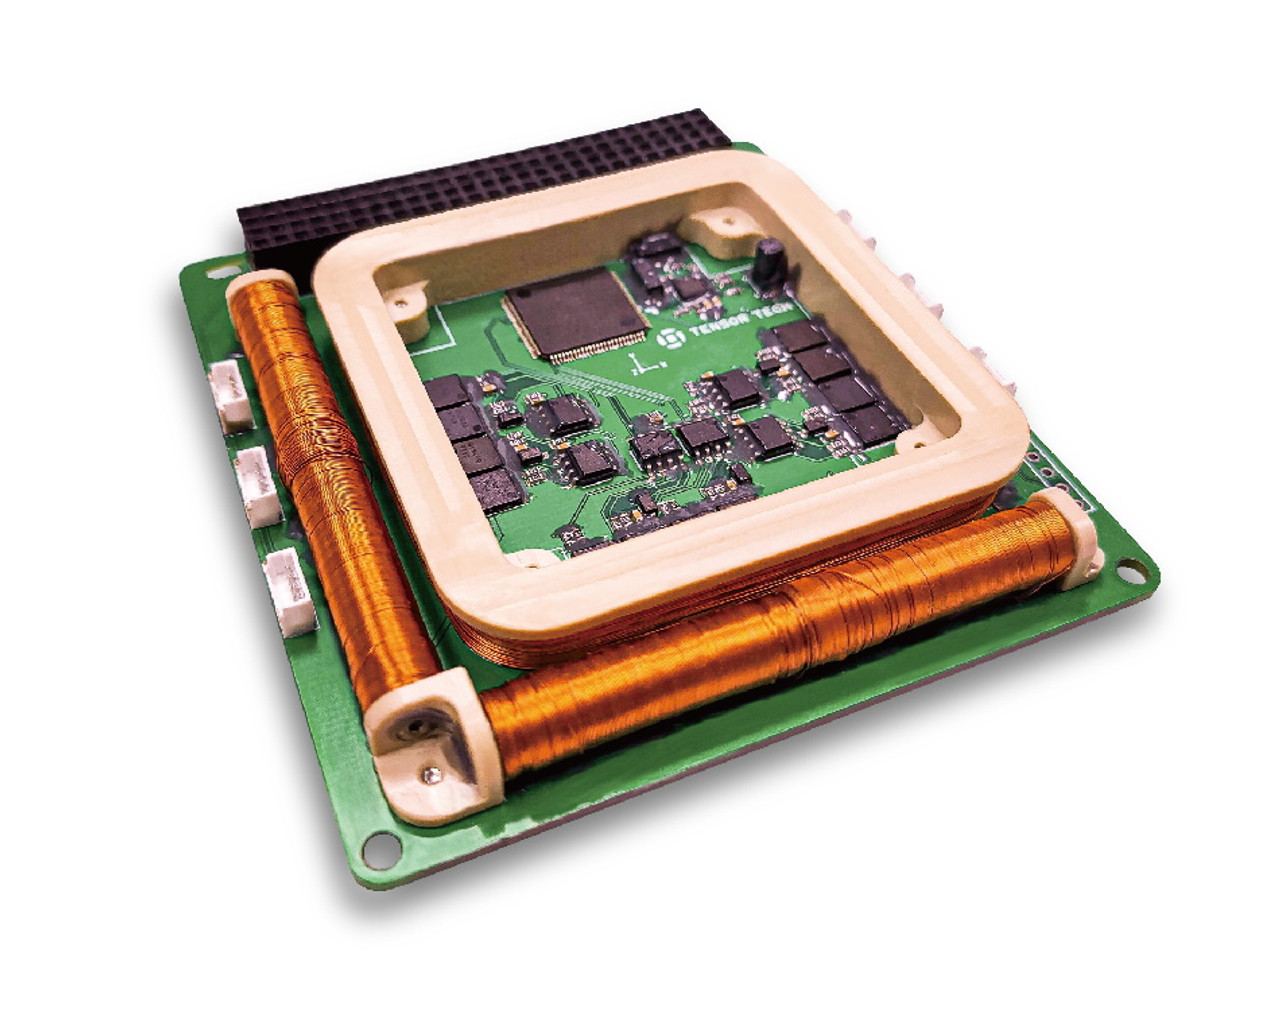
\includegraphics[width=0.5\textwidth]{./Figures/ADCS-Commercial.jpg}
	\caption{ADCS comercial - modelo ADCS-MTQ.}
	\label{fig:adcs_commercial}
\end{figure}


El sistema ADCS se encarga de mantener y corregir  la orientación del satélite a una orientación mediante un algoritmo de control. 

Un sistema ADCS consta de una unidad inercial de medición(IMU por sus siglas en inglés). Este dispositivo mide campo magnético, aceleración y velocidad angular en tres ejes. 
Con estos datos  determina la orientación dentro del espacio usando algoritmos como TRIAD, Davenports, entre otros.
Una vez calculada la orientación, el sistema genera una actuación (por ejemplo, mediante magnetorqueres o ruedas de reacción) para aplicar un torque (o par) en alguno de los ejes principales. Esto permite mantener la orientación deseada y compensar perturbaciones externas, como la resistencia atmosférica o la influencia gravitatoria. 


\section{Estado del Arte}

El control de actitud en vehículos espaciales es un área ampliamente estudiada, con múltiples enfoques que combinan sensores, algoritmos de estimación y actuadores para mantener o modificar la orientación del vehículo en el espacio. Existen diversas plataformas de simulación y validación de sistemas ADCS, muchas de ellas desarrolladas en entornos como MATLAB/Simulink, FreeFlyer, o STK. Sin embargo, estas soluciones presentan ciertas limitaciones, especialmente en contextos educativos o de bajo presupuesto.

Durante la etapa inicial de esta tesis se realizó una revisión exploratoria de herramientas disponibles, lo cual permitió identificar algunas dificultades frecuentes. Por un lado, muchas plataformas requieren licencias costosas, lo que puede restringir su uso en entornos académicos. Por otro, su complejidad técnica y curva de aprendizaje representan una barrera para estudiantes o investigadores que se inician en esta área. 

Además, se observó que pocas de estas herramientas permiten integración directa con microcontroladores u otros sistemas embebidos, lo cual complica la validación práctica de los algoritmos desarrollados. Del mismo modo, en varios casos la simulación de sensores se realiza bajo condiciones ideales, sin considerar la presencia de ruido, que limita la validez del modelo en entornos reales. 

Frente a estas limitaciones, el desarrollo propuesto en esta tesis busca ofrecer una alternativa accesible, de bajo costo y fácil de utilizar, que permita tanto la simulación como la conexión directa con hardware físico. Entre sus características, se destaca la capacidad de simular sensores con ruido, modificar algoritmos y configuraciones de sensores de manera modular, y validar los resultados directamente sobre un microcontrolador. Esto proporciona un entorno de desarrollo más realista y adaptable, especialmente útil en entornos educativos o de investigación aplicada. 



\section{Desarrollo del trabajo}
	El trabajo desarrolla la simulación de un control de actitud utilizando el algoritmo TRIAD para estimar la orientación del satelite. Este método compara dos referencias conocidas (por ejemplo campo magnético, aceleración de la gravedad, dirección del sol, etc) con las mediciones de los sensores a bordo. A partir de esta comparación,el TRIAD determina la orientación relativa del Cubesat respecto a un sistema de coordenadas de referencia. El diagrama en bloques del trabajo desarrollado se muestra a continuación: 
	\begin{figure}[htbp]
		\centering
		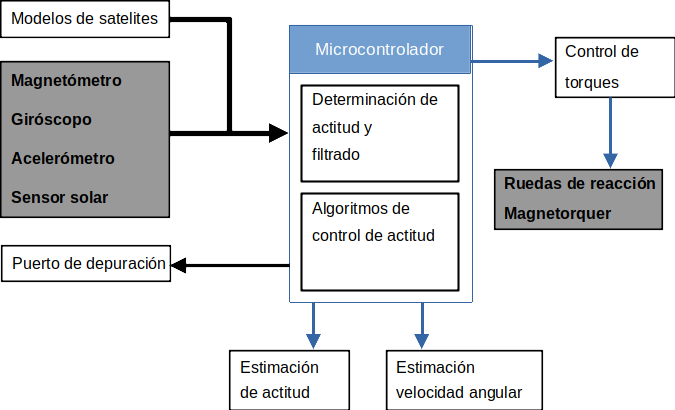
\includegraphics[width=0.7\textwidth]{./Figures/sistemaadcs.png}
		\caption{Diagrama en bloques del trabajo desarrollado.}
		\label{fig:simulate_sistem}
	\end{figure}

	El desarrollo de los algoritmos se realizó en dos lenguajes de programación: C para la implementación embebida y Python para prototipado rápido y validación de modelos. El código en C se integrará en un sistema embebido utilizando la metodología HIL (Hardware-in-the-Loop), que permite validar el comportamiento del sistema de control en un entorno simulado antes de su implementación física.





\section{Objetivos}

El objetivo inicial del proyecto consistía en desarrollar una placa de circuito impreso (PCB) con sistemas de actuación para control de actitud, ya sea mediante ruedas de reacción o magnetorquers. Sin embargo, durante la fase inicial de desarrollo se identificaron varias limitaciones significativas:

\begin{itemize}
	\item \textbf{Alto costo de soluciones comerciales}: Los modelos existentes para simulación presentaban costos prohibitivos para instituciones académicas.
	\item \textbf{Limitaciones en software libre}: Las herramientas analizadas (GMAT, Octave, entre otros) carecían de capacidad nativa para integración HIL (Hardware-in-the-Loop) con microcontroladores, siendo Matlab la única alternativa viable pero con sus propias dificultades técnicas.
	\item \textbf{Barreras económicas}: Los costos asociados a las soluciones comerciales resultaban inviables para su implementación en el contexto universitario.
\end{itemize}
Estos hallazgos motivaron una ampliación del alcance del trabajo, incorporando los siguientes objetivos tecnicos:

\begin{itemize}
	\item Desarrollo de un modelo dinámico de simulación que incluya:
	\begin{itemize}
		\item Modelado matemático del satélite y su entorno orbital
		\item Simulación de sensores (generación de datos sintéticos)
	\end{itemize}
	\item Implementación de una plataforma HIL que permita:
	\begin{itemize}
		\item Conexión con hardware real (microcontrolador/procesador)
		\item Inyección de datos de sensores simulados al sistema embebido
		\item Validación de los algoritmos de control en condiciones emuladas
	\end{itemize}
\end{itemize}


Este enfoque permitirá evaluar el rendimiento del sistema de control antes de proceder al diseño final del circuito impreso, reduciendo riesgos técnicos y costos asociados a iteraciones de hardware. Cabe aclarar que la simulación parte del supuesto de que el sistema ya se encuentra en la órbita deseada, sin modelar el proceso de inserción orbital ni el trayecto previo.





	\chapter{Introducción específica} % Main chapter title

\label{Chapter2}

%----------------------------------------------------------------------------------------
%	SECTION 2 resume 
%----------------------------------------------------------------------------------------
Se presentan las bases matemáticas del control de actitud. El control de actitud se basa en seleccionar al menos dos sistemas de referencia para definir las orientaciones a través de una matriz. Al seleccionarse dos referencias puede utilizarse diferentes parametrizaciónes de la matriz: 
\begin{itemize}
	\item Quaterniones
	\item Parámetros de Rodrigues
	\item Parámetros de Euler
	\item Parámetros de Rodrigues modificado.
	\item etc,,, 
\end{itemize}
Esta parametrización presenta ventajas sobre la matriz. La idea central del control de actitud es estimar la matriz de orientaciones. EN este contexto la matriz se llama \"matriz de Actitude\". Esta matriz se obtiene a partir de la parametrización y del modelo dinámico del sistema, donde lo que se obtiene es una estimación y no la matriz real, según el algoritmo utilizado 
 

\section{Estilo y convenciones}
\label{sec:ejemplo}

\subsection{Rotaciones activas vs Pasivas}


 
	\include{Chapters/Chapter3}
	\include{Chapters/Chapter4} 
	\include{Chapters/Chapter5} 
\end{verbatim}

Los apéndices también deben escribirse en archivos .tex separados, que se deben ubicar dentro de la carpeta \emph{Appendices}. Los apéndices vienen comentados por defecto con el caracter \code{\%} y para incluirlos simplemente se debe eliminar dicho caracter.

Finalmente, se encuentra el código para incluir la bibliografía en el documento final.  Este código tampoco debe modificarse. La metodología para trabajar las referencias bibliográficas se desarrolla en la sección \ref{sec:biblio}.
%----------------------------------------------------------------------------------------

\section{Bibliografía}
\label{sec:biblio}

Las opciones de formato de la bibliografía se controlan a través del paquete de latex \option{biblatex} que se incluye en la memoria en el archivo memoria.tex.  Estas opciones determinan cómo se generan las citas bibliográficas en el cuerpo del documento y cómo se genera la bibliografía al final de la memoria.

En el preámbulo se puede encontrar el código que incluye el paquete biblatex, que no requiere ninguna modificación del usuario de la plantilla, y que contiene las siguientes opciones:

\begin{lstlisting}
\usepackage[backend=bibtex,
	natbib=true, 
	style=numeric, 
	sorting=none]
{biblatex}
\end{lstlisting}

En el archivo \file{reference.bib} se encuentran las referencias bibliográficas que se pueden citar en el documento.  Para incorporar una nueva cita al documento lo primero es agregarla en este archivo con todos los campos necesario.  Todas las entradas bibliográficas comienzan con $@$ y una palabra que define el formato de la entrada.  Para cada formato existen campos obligatorios que deben completarse. No importa el orden en que las entradas estén definidas en el archivo .bib.  Tampoco es importante el orden en que estén definidos los campos de una entrada bibliográfica. A continuación se muestran algunos ejemplos:

\begin{lstlisting}
@ARTICLE{ARTICLE:1,
    AUTHOR="John Doe",
    TITLE="Title",
    JOURNAL="Journal",
    YEAR="2017",
}
\end{lstlisting}


\begin{lstlisting}
@BOOK{BOOK:1,
    AUTHOR="John Doe",
    TITLE="The Book without Title",
    PUBLISHER="Dummy Publisher",
    YEAR="2100",
}
\end{lstlisting}


\begin{lstlisting}
@INBOOK{BOOK:2,
    AUTHOR="John Doe",
    TITLE="The Book without Title",
    PUBLISHER="Dummy Publisher",
    YEAR="2100",
    PAGES="100-200",
}
\end{lstlisting}


\begin{lstlisting}
@MISC{WEBSITE:1,
    HOWPUBLISHED = "\url{http://example.com}",
    AUTHOR = "Intel",
    TITLE = "Example Website",
    MONTH = "12",
    YEAR = "1988",
    URLDATE = {2012-11-26}
}
\end{lstlisting}

Se debe notar que los nombres \emph{ARTICLE:1}, \emph{BOOK:1}, \emph{BOOK:2} y \emph{WEBSITE:1} son nombres de fantasía que le sirve al autor del documento para identificar la entrada. En este sentido, se podrían reemplazar por cualquier otro nombre.  Tampoco es necesario poner : seguido de un número, en los ejemplos sólo se incluye como un posible estilo para identificar las entradas.

La entradas se citan en el documento con el comando: 

\begin{verbatim}
\citep{nombre_de_la_entrada}
\end{verbatim}

Y cuando se usan, se muestran así: \citep{ARTICLE:1}, \citep{BOOK:1}, \citep{BOOK:2}, \citep{WEBSITE:1}.  Notar cómo se conforma la sección Bibliografía al final del documento.

Finalmente y como se mencionó en la subsección \ref{subsec:configurando}, para actualizar las referencias bibliográficas tanto en la sección bibliografía como las citas en el cuerpo del documento, se deben ejecutar las herramientas de compilación PDFLaTeX, BibTeX, PDFLaTeX, PDFLaTeX, en ese orden.  Este procedimiento debería resolver cualquier mensaje "Citation xxxxx on page x undefined".
